\documentclass{article}
\usepackage[utf8]{inputenc}
\usepackage{graphicx} % Required for inserting images
\graphicspath{ {./images/} }
\usepackage{mathtools} % for math tool slike arrows

\title{Introduction to Quantum Information and Computing Half 2 Lecture 3}
\author{Shrikara A, Arnav Negi, Kriti Gupta, Manav Shah, Mohammed Shamil,\\ Shiven Sinha, Swayam Agarwal, Vineeth Bhat, Yash Adivarekar}
\date{17th February, 2023}

\begin{document}

\maketitle

\section{Tofolli Gate}

Also known as $CCNOT$ Gate.

\begin{figure}[htp]
    \centering
    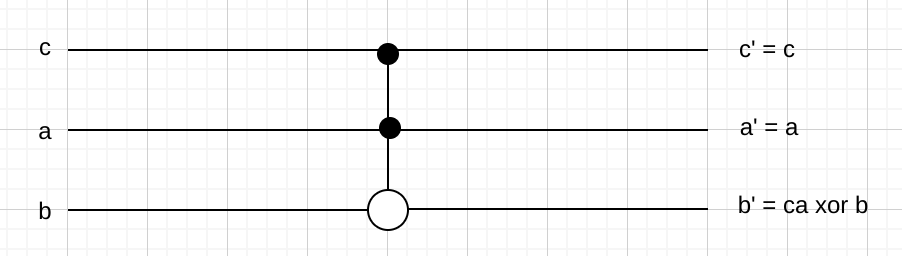
\includegraphics[width=10cm]{tofolli.png}
\end{figure}

The $CCNOT$ gate preserves the control, $c$, and first input, $a$, and only performs an operation on the last input, $b$, to give the output $$b'=ca \oplus b$$

which means that for $b$ to be flipped, both $a$ and $c$ must be 1.

Further, this gate is universal and reversible.

\section{Some problems}

\begin{enumerate}
    \item We receive some garbage bits that we don't require in the output of a quantum gate. For example, consider the operation carried out by a unitary $u_f$:
    $$|x,0,0\rangle \xrightarrow[]{u_f} \Sigma_y \alpha |y\rangle |f(y)\rangle |g(y)\rangle $$
    The term $|g(y)\rangle$ might not be needed and is termed as garbage or ancillary.
    \item The garbage bits are entangled with the input and cannot be reset as it will make the operation irreversible.
    \item We cannot measure the garbage register either as measurement will collapse the superposition to a particular state which isn't desirable.
\end{enumerate}
This is solved using uncomputation.

\section {Uncomputation}

Say we wish to obtain the solution $|f(x)\oplus y \rangle$ given the inputs $|x\rangle$ and $|y\rangle$ as follows:

$$|x\rangle |0\rangle |0\rangle |y\rangle \xrightarrow[]{u_f} |x\rangle |f(x)\rangle |g(x)\rangle |y\rangle$$

Where the unitary $u_f$ is applied on the first three qubits.

$$|x\rangle |f(x)\rangle |g(x)\rangle |y\rangle \xrightarrow[]{CNOT_{2,4}} |x\rangle |f(x)\rangle |g(x)\rangle |f(x) \oplus y\rangle$$

We then use the $CNOT$ gate on the 2nd and 4th qubits, i.e., $|f(x)\rangle$ and $|y\rangle$

$$|x\rangle |f(x)\rangle |g(x)\rangle |f(x) \oplus y\rangle \xrightarrow[]{u^{-1}_f} |x\rangle |0\rangle |0\rangle |f(x) \oplus y\rangle$$

We use the inverse of the unitary operation used earlier to uncompute the 2nd and 3rd bits.

All of these operations are represented by the short hand notation:

\begin{figure}[htp]
    \centering
    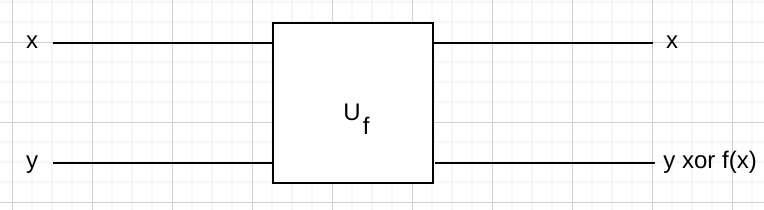
\includegraphics[width=10cm]{uncomputation.png}
\end{figure}

\section {Quantum Circuits}

We note that
\begin{enumerate}
    \item Quantum gates are unitary operations on quantum states.
    \item There exists a set of universal gates for quantum circuits usually denoted by $G_O$, which contains a small number of single as well as two qubit gates.
\end{enumerate}

\subsection{Single Qubit Gates}

These include 

\begin{enumerate}
    \item Pauli matrices (which have been elucidated on earlier in the first half)
    \item Hadamard matrix

    $$H = \frac{1}{\sqrt{2}} \begin{bmatrix}
            1 & 1\\
            1 & -1
    \end{bmatrix}$$

    They transform from the basis $\{|0\rangle, |1\rangle\}$ to $\{|+\rangle, |-\rangle\}$.

    $$H|0\rangle = |+\rangle = \frac{1}{\sqrt{2}}(|0\rangle + |1\rangle)$$    
    $$H|1\rangle = |-\rangle = \frac{1}{\sqrt{2}}(|0\rangle - |1\rangle)$$    
    
    \item Phase change matrices

    $$R_{\phi} = \begin{bmatrix}
            1 & 0\\
            0 & e^{i\phi}    
    \end{bmatrix}$$

    The phase change matrix adds a change of phase $\phi$ to the the state $|1\rangle$ as $$R_{\phi}(|\alpha |0\rangle + \beta |1\rangle) = |\alpha |0\rangle + e^{i\phi}\beta |1\rangle$$

    Some accepted ways of denoting common phase changes are $S=R_{\frac{\pi}{2}}$ and $T=R_{\frac{\pi}{4}}$.
    
\end{enumerate}

\subsection{Two Qubit Gates}

\subsubsection{Controlled two qubit gates}

For example, if we wish to apply the unitary $u$ only on the second state in $|ab\rangle$, i.e., as a $controlled$ operation on a single qubit gate, we use the circuit:

\begin{figure}[htp]
    \centering
    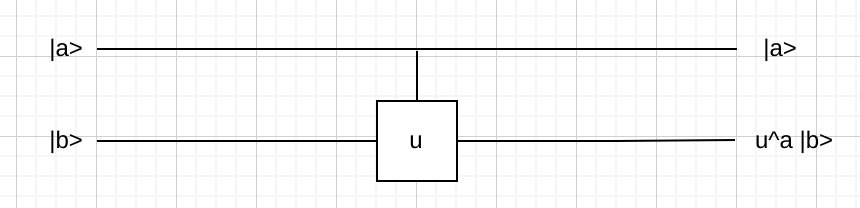
\includegraphics[width=10cm]{twoqubit.png}
\end{figure}

The matrix representation of the operation is

$$
    U = \begin{bmatrix}
        \begin{matrix}
            1 && 0\\
            0 && 1
        \end{matrix}
        && 
        \begin{matrix}
            0 && 0\\
            0 && 0
        \end{matrix}
        \\
        \begin{matrix}
            0 && 0\\
            0 && 0
        \end{matrix}
        && 
        u
    \end{bmatrix}
$$

The operations carried out are:
$$|00\rangle \xrightarrow[]{U} |00\rangle$$
$$|01\rangle \xrightarrow[]{U} |01\rangle$$
$$|10\rangle \xrightarrow[]{U} |1\rangle(u|0\rangle)$$
$$|11\rangle \xrightarrow[]{U} |1\rangle(u|1\rangle)$$

For example, if we wish to model the $CNOT$ gate, we take $u=\sigma _x$ if the above circuit.

\subsubsection{Another example of two qubit gates}

Consider the following circuit

\begin{figure}[htp]
    \centering
    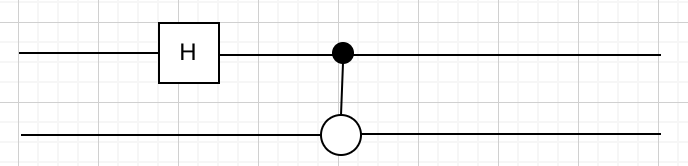
\includegraphics[width=10cm]{extwoqubit.png}
\end{figure}

If we apply this circuit on the input $|00\rangle$, then we can model the output using the following calculations

$$|00\rangle \xrightarrow[]{H \otimes \mathbf{I}} |+0\rangle = \frac{1}{\sqrt{2}}(|00\rangle + |10\rangle)$$

$$\frac{1}{\sqrt{2}}(|00\rangle + |10\rangle) \xrightarrow[]{CNOT} \frac{1}{\sqrt{2}}(|00\rangle + |11\rangle)$$

\end{document}